% !TEX encoding = UTF-8
% !TEX program = xelatex
\documentclass[12pt,a4paper]{article}
\usepackage[paperwidth=210mm, paperheight=297mm, left=0.75in, right=0.75in, bottom=1in, top=1in]{geometry}
\usepackage{polyglossia}
\setdefaultlanguage[babelshorthands]{italian}
\usepackage{fontspec}
\usepackage{graphicx}
\usepackage{blindtext}
\usepackage{wrapfig}

\frenchspacing
\makeindex

\begin{document}
\title{\vspace{-70pt}Planck}
\author{Francesco Zanini}
\date{}
\maketitle
\pagestyle{empty}
\thispagestyle{empty}

\section*{Storia}
\begin{wrapfigure}{r}{0.35\textwidth}
  \vspace{-10pt}
  \begin{center}
    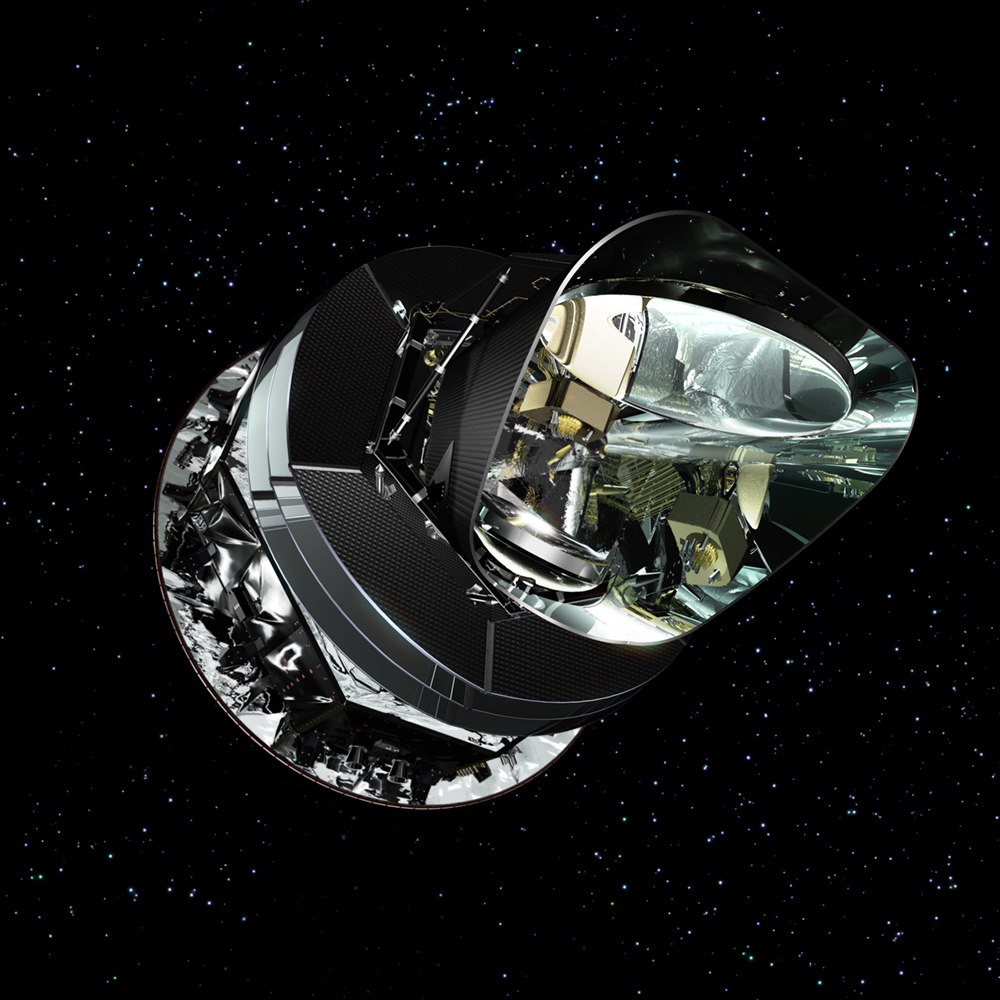
\includegraphics[width=0.30\textwidth]{satellite}
  \end{center}
  \vspace{-20pt}
\end{wrapfigure}
Il satellite Planck è stato inviato nello spazio nel mese di Maggio 2009 dalla base di lancio di Kourou, situata in America del Sud, vicino all'Equatore. Il lanciatore era un \emph{Ariane 5 ECA}, l'ultimo modello dei lanciatori gestiti dall'Agenzia Spaziale Europea (ESA) e dall'ente spaziale francese (CNES).

La destinazione di Planck è il \emph{punto lagrangiano L2}, posizionato a 1,5 milioni di Km dalla Terra in direzione opposta al Sole. L2 è un \emph{punto di equilibrio del campo gravitazionale} combinato della Terra e del Sole e nel corso dell'anno si muove insieme alla Terra attorno al Sole, mantenendo sempre la stessa posizione rispetto alla Terra.

Il punto lagrangiano L2 offre diversi vantaggi per missioni di osservazione dell'Universo, in particolare per le misure di Fondo Cosmico a Microonde, è stato già infatti sfruttato dalla missione WMAP:
\begin{itemize}
\item \emph{l'allineamento di Sole e Terra} nell'arco di pochi gradi, nel caso particolare di Planck 10°, permette di avere un ampio campo di vista senza rischio di interferenza da parte di emissione solare o terrestre;
\item la \emph{continua esposizione al Sole}, sempre nella medesima angolazione e distanza, permette sia di avere alimentazione continua per i pannelli solari, ma soprattutto garantire minime fluttuazioni termiche dovute a variazioni di temperatura;
\item la \emph{notevole distanza dalla Terra} permette di ridurre le interferenze sia di emissione di calore che di onde elettromagnetiche anche se complica la trasmissione di dati alle stazioni di Terra.
\end{itemize}

\section*{Osservazioni}
Un aspetto molto importante per Planck, e in generale per molti esperimenti di fondo cosmico (CMB) e osservazioni astronomiche, è il \emph{modo in cui viene osservato il cielo}.

Planck è un satellite che \emph{ruota attorno al suo asse} (si parla di ``spinning satellite'') una volta al minuto. L'asse ottico del telescopio di Planck punta a 85 gradi dall'asse di rotazione del satellite. Allora, per ogni direzione dell'asse di rotazione del satellite, il telescopio di Planck osserva un grande cerchio nel cielo. In realtà ogni rivelatore di Planck punta in una sua specifica direzione distante solo pochi gradi da quella dell'asse del telescopio: perciò \emph{ogni rivelatore osserva il proprio particolare cerchio in cielo}.

Riordinando le osservazioni prese cerchio per cerchio si costruisce la \emph{mappa del cielo} per ogni rivelatore. Combinando insieme i dati e le mappe di tutti i rivelatori che operano alla stessa frequenza di osservazione si ottiene la mappa finale a ciascuna frequenza osservata da Planck. Queste mappe alle 9 frequenze vengono analizzate insieme per ottenere la mappa delle\emph{ anisotropie} del CMB e quelle di tutte le altre \emph{componenti astrofisiche}.
\end{document}